\documentclass{beamer}

\usepackage{framed}
\usepackage{graphicx}

\begin{document}
%====================================%
\begin{frame}[fragile]
\frametitle{Seaborn Workshop}
\large

To remedy this, seaborn provides an interface to the husl system, which also makes it easy to select evenly spaced hues while keeping the apparent brightness and saturation much more uniform.
\begin{verbatim}
sns.palplot(sns.color_palette("husl", 8))
\end{verbatim}

\begin{figure}
\centering

\includegraphics[width=0.7\linewidth]{images/color_palettes_14_0}
\caption{}
\label{fig:color_palettes_14_0}
\end{figure}

There is similarly a function called \texttt{husl\_palette()} that provides a more flexible interface to this system.
\end{frame}
\section{Using categorical Color Brewer palettes}
%====================================%
\begin{frame}[fragile]
	\frametitle{Seaborn Workshop}
	\large
\textbf{Using categorical Color Brewer palettes}
Another source of visually pleasing categorical palettes comes from the Color Brewer tool (which also has sequential and diverging palettes, as we’ll see below). These also exist as matplotlib colormaps, but they are not handled properly. In seaborn, when you ask for a qualitative Color Brewer palette, you’ll always get the discrete colors, but this means that at a certain point they will begin to cycle.
\end{frame}
%====================================%
\begin{frame}[fragile]
	\frametitle{Seaborn Workshop}
	\large
	\begin{itemize}
\item A nice feature of the Color Brewer website is that it provides some guidance on which palettes are color blind safe. 
\item There are a variety of [kinds](http://en.wikipedia.org/wiki/Color\_blindness) of color blindness, but the most common variant leads to difficulty distinguishing reds and greens.
\item It’s generally a good idea to avoid using red and green for plot elements that need to be discriminated based on color.
\end{itemize}
\end{frame}
%====================================%
\begin{frame}[fragile]
	\frametitle{Seaborn Workshop}
	\large
\begin{verbatim}
sns.palplot(sns.color_palette("Paired"))
\end{verbatim}

\begin{figure}
\centering

\includegraphics[width=0.7\linewidth]{images/color_palettes_16_0}
\caption{}
\label{fig:color_palettes_16_0}
\end{figure}
\end{frame}
%====================================%
\begin{frame}[fragile]
	\frametitle{Seaborn Workshop}
	\large
\begin{verbatim}
sns.palplot(sns.color_palette("Set2", 10))
\end{verbatim}
\begin{figure}
\centering

\includegraphics[width=0.7\linewidth]{images/color_palettes_17_0}
\caption{}
\label{fig:color_palettes_17_0}
\end{figure}
\end{frame}
%====================================%
\begin{frame}[fragile]
	\frametitle{Seaborn Workshop}
	\large
	\begin{itemize}
\item To help you choose palettes from the Color Brewer library, there is the \texttt{choose\_colorbrewer\_palette()} function.
\item This function, which must be used in an IPython notebook, will launch an interactive widget that lets you browse the various options and tweak their parameters.
	\end{itemize}

\end{frame}
%====================================%
\begin{frame}[fragile]
\frametitle{Seaborn Workshop}
\large

Of course, you might just want to use a set of colors you particularly like together. Because \texttt{color\_palette()} accepts a list of colors, this is easy to do.
\begin{verbatim}
flatui = ["#9b59b6", "#3498db", "#95a5a6", "#e74c3c", "#34495e", "#2ecc71"]
sns.palplot(sns.color_palette(flatui))
\end{verbatim}
\begin{figure}
	\centering
	
\includegraphics[width=0.7\linewidth]{images/color_palettes_19_0}
\end{figure}
\end{frame}
\section{Using named colors from the xkcd color survey}
	
%====================================%
\begin{frame}[fragile]
	\frametitle{Seaborn Workshop}
	\large
A while back, xkcd ran a crowdsourced effort to name random RGB colors. This produced a set of 954 named colors, which you can now reference in seaborn using the \texttt{xkcd\_rgb} dictionary:
\begin{verbatim}
plt.plot([0, 1], [0, 1], sns.xkcd_rgb["pale red"], lw=3)
plt.plot([0, 1], [0, 2], sns.xkcd_rgb["medium green"], lw=3)
plt.plot([0, 1], [0, 3], sns.xkcd_rgb["denim blue"], lw=3);
\end{verbatim}

\begin{figure}
\centering
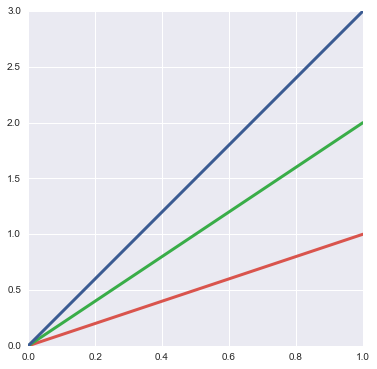
\includegraphics[width=0.7\linewidth]{images/color_palettes_21_0}
\caption{}
\label{fig:color_palettes_21_0}
\end{figure}
\end{frame}
%====================================%
\begin{frame}[fragile]
	\frametitle{Seaborn Workshop}
	\large
If you want to spend some time picking colors, this interactive visualization may be useful. In addition to pulling out single colors from the \texttt{xkcd\_rgb} dictionary, you can also pass a list of names to the \texttt{xkcd\_palette()} function.
\begin{verbatim}

colors = ["windows blue", "amber", "greyish", "faded green", "dusty purple"]
sns.palplot(sns.xkcd_palette(colors))
\end{verbatim}

\begin{figure}
\centering

\includegraphics[width=0.7\linewidth]{images/color_palettes_23_0}
\caption{}
\label{fig:color_palettes_23_0}
\end{figure}

\end{frame}

\end{document}